\icode{E-MD-CA-L3-261111-002}
如图所示，质量为 \(m_0 =\) \,\qty{4}{kg}的木板长 \(L =\) \,\qty{1.4}{m}，静止放在光滑的水平地面上，其右端静置一质量为 \(m =\) \,\qty{1}{kg}的小滑块（可视为质点），小滑块与木板间的动摩擦因数 \(\mu = 0.4\)，今用水平力 \(F =\) \,\qty{28}{N}向右拉木板，要使小滑块从木板上掉下来，力 \(F\) 作用的时间至少要多长？（不计空气阻力，\(g =\) \,\qty{10}{m/s^2}）

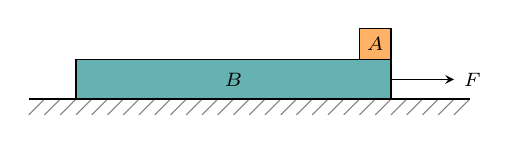
\begin{tikzpicture}[>=stealth,font=\scriptsize]
	\draw[fill=teal!60] (0,0) rectangle(4,.5)node[midway]{\(B\)};
	\draw[fill=orange!60] (3.6,.5) rectangle(4,.9)node[midway]{\(A\)};
	\draw[->] (4,.25)--++(.8,0)node[right]{\(F\)};
	\foreach \x in {-.6,-.4,...,5}
		\draw[gray] (\x,-.2)--++(.2,.2);
	\draw[thick] (-.6,0)--(5,0);
\end{tikzpicture}
\begin{answer}
    \qty{1}{s}
\end{answer}